\section{Aufbau und Durchführung}
\label{sec:Durchführung}
Für die im folgendem beschriebenen Versuchsteile wird der in Abbildung \ref{fig:Aufbau} verwendete Aufbau verwendet.
\begin{figure}[H]
  \centering
  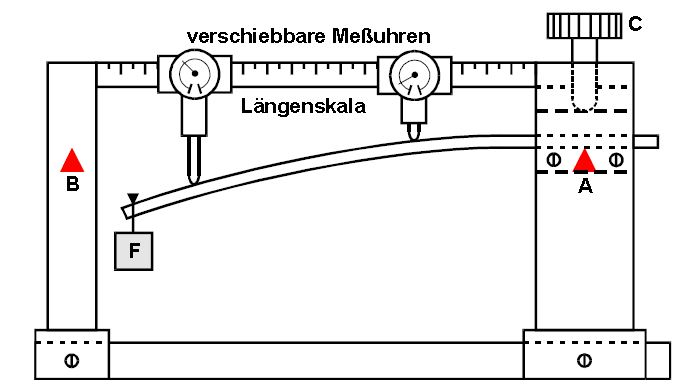
\includegraphics[scale=0.7]{Text/Bilder/Aufbau.jpg}
  \caption{Skizze der Messapparatur\cite[226]{sample}}
  \label{fig:Aufbau}
\end{figure}
Dieser besteht aus einer Probe, die in eine Bleiabschirmung gesteckt wird, einem Verstärker, zwei Zählern, einer Spannungsversorgung und einem Zeitgeber.
Neben der Probe befindet sich ein Zählrohr,
welches die durch die eintreffende Strahlung entstehenden Impulse über einen Verstärker an die Zähler weitergibt.
Am Zeitgeber kann eingestellt werden, wie lange der Messvorgang laufen soll. \newline

Im ersten Versuchsteil wird eine Nulleffektmessung durchgeführt. Dazu wird, ohne die Verwendung einer Probe, in einem Zeitraum von $\symup{\Delta} t= \SI{900}{\second}$ eine Messung durchgeführt.
Im nächsten Versuchteil wird daraufhin die Halbwertszeit des Elementes $\ce{^{116}In}$ untersucht. Dazu werden in einem Intervall von $\symup{\Delta} t= \SI{240}{\second}$ die Anzahl der
aufgenommenden elekrischen Impulse für einen Zeitraum von $60$ Minuten gemessen.
Dies wird für ein Isomerengemisch von $\ce{^{104}Rh}$ und $\ce{^{104i}Rh}$ wiederholt. Aufgrund der kurzen Halbwertszeit von $\ce{^{104}Rh}$ muss das Messintervall hier jedoch auf
$\symup{\Delta} t= \SI{18}{\second}$ reduziert werden. Es werden $42$ Messwerte aufgenommen.
